\section{Aufbau}
\label{sec:Aufbau}
Der Versuchaufbau ist in \autoref{fig:Aufbau} dargestellt und besteht hauptsächlich aus einer $\gamma$-Quelle, einem Würfel und einem NaJ-Detektor.
\begin{figure}[H]
    \centering
    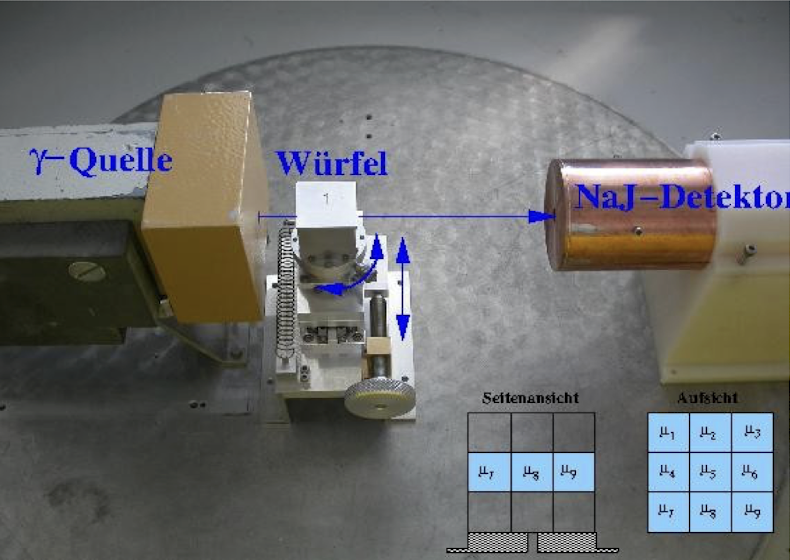
\includegraphics[scale=0.7]{Abbildungen/Aufbau.png}
    \caption{Bild von dem Versuchsaufbau.\cite{V14}}
    \label{fig:Doppelbrechung}
\end{figure}
Die $\gamma$-Quelle sendet einen kollimierten Strahl aus, welcher auf den Würfel trifft. 
Der Würfel ist $\qty{3}{\centi\meter} \times \qty{3}{\centi\meter} \times \qty{3}{\centi\meter}$ groß und besteht aus $3 \times 3 \times 3$ Elementarwürfeln, die eime Seitenlänge
von $\qty{1}{\centi\meter}$ besitzen. Die Elemantarwürfel werden von einer Aluminiumhülle umgeben mit einer Wandstärke von $\qty{1}{\milli\meter}$.\\
Es gibt vier Arten von diesen Würfel. Der erste Würfel ist nur die Aluminiumhülle. Der zweite und dritte Würfel besteht nur aus einem Material. Der vierte Würfel besteht aus
einer Mischung von Elementarwürfeln der Materialen des zweiten und dritten Würfel.
Der Würfel kann um seine z-Achse gedreht werden und senkrecht zu der strahlrichtung verschoben werden.
Der Strahl wird nach dem durchlaufen des Würfels von einem NaJ-Detektor aufgenommen, wobei die vom Sizintillatordetektor erzeugten Pulse von einem Vorverstärker verstärkt werden.
Anschließend werden diese Pulse von einem Multichannelanalyser analysiert, indem das Siganl entsprechend seiner Größe einen Kanal innerhalb des Datensatzes zugeordnet wird.
An einem Spektroskopie Amplifier werde die Detektorspannung und die Vorverstärkerspannung eingestellt und die Diskriminatorschwelle und die Datenaufnahme werden über den Computer und einem 
Programm ausgewertet.


\section{Durchführung}
\label{sec:Durchführung}
Zuerst wird das Spektrum der Quelle bestimmt, ohne Abschwächung des Strahls. Dabei sollen alle Prozesse des Spektrums identifiziert werden.
Es wird über einem Zeitraum  von $t = \qty{300}{\second}$ gemessen.
Anschließend wird die Messung mit den vier Würfeln durchgeführt und die Werte aufgenommen.
Es wird nur die mittlere Schicht des Würfels untersucht, aufgrund von Zeitgründen.  Bei den homogenen Würfeln wird aus vier Richtungen gemessen, wobei der Würfel mit den verschiedenen 
Elementarwürfeln wird aus allen 12 Richtungen gemessen wird (siehe \autoref{fig:Ausrichtung}).